\documentclass{standalone}
\usepackage{pgfplots}
\pgfplotsset{compat=1.18}
\usepackage{xcolor}
\begin{document}
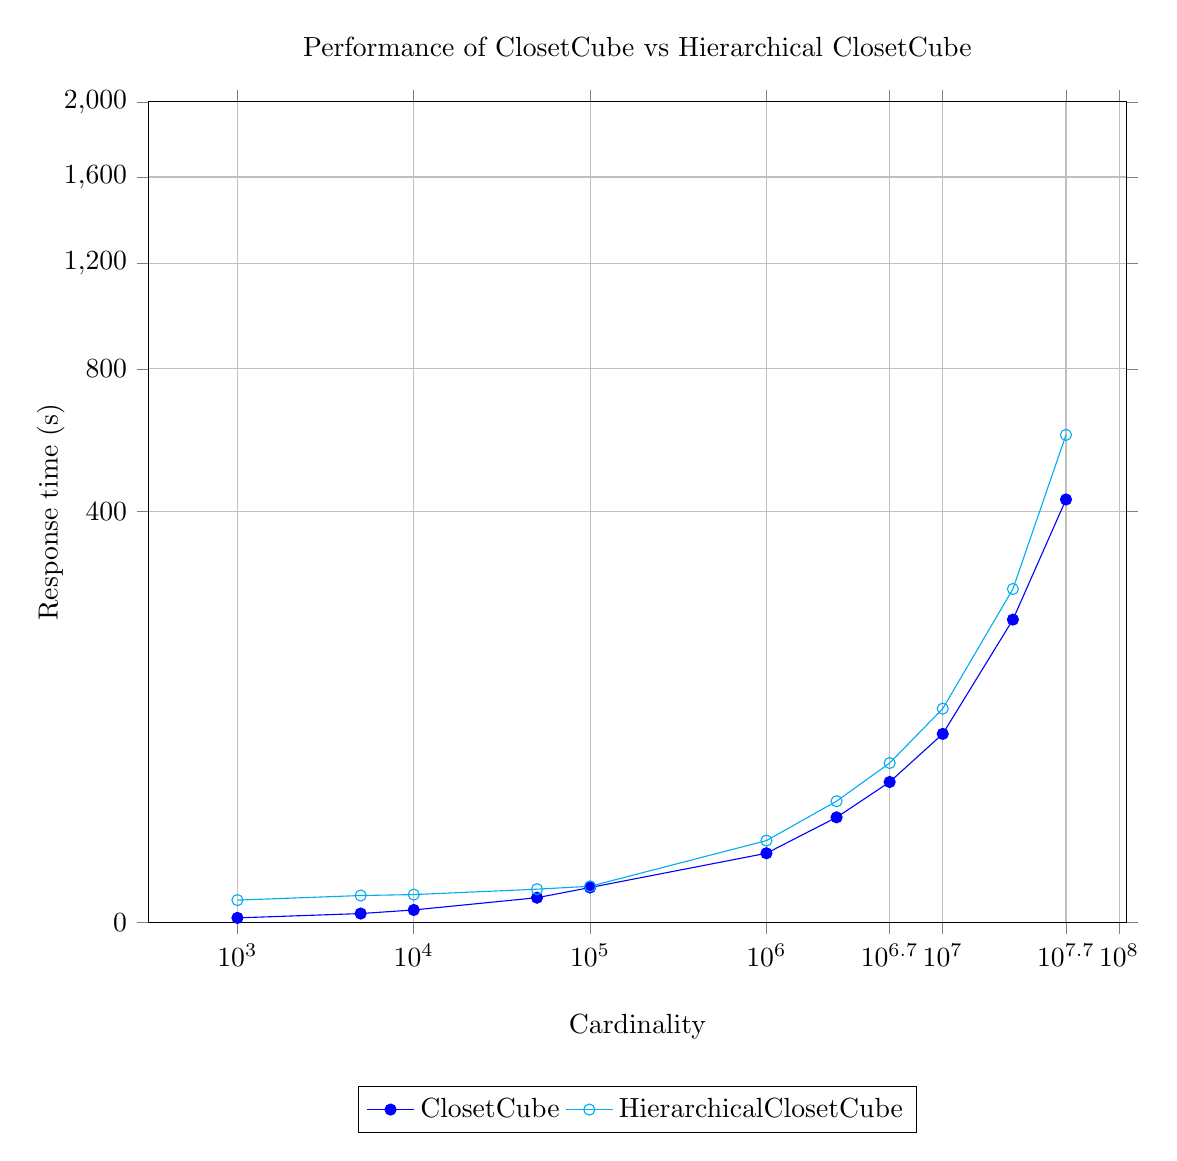
\begin{tikzpicture}
\begin{axis}[
xlabel={Cardinality},
ylabel={Response time (s)},
title={Performance of ClosetCube vs Hierarchical ClosetCube},
title style={yshift=0.7em},
ymode=linear,
y coord trafo/.code={ \pgfmathparse{ (max(#1, 1e-09)/2000)^0.43 } \pgfmathresult },
y coord inv trafo/.code={ \pgfmathparse{ (max(#1, 1e-09)^2.3255813953488373) * 2000 } \pgfmathresult },
ymin=0, ymax=2000,
y label style={at={(axis description cs:-0.1,0.5)},anchor=center},
yticklabel style={/pgf/number format/fixed, /pgf/number format/precision=0},
ytick={ 0,399,800,1199,1599,2000 },
minor y tick num=0,
xmode=log, log basis x=10,
xtick={ 1000,10000,100000,1000000,5000000,10000000,50000000,100000000 },
xmax=110000000.00000001,
xticklabel style={/pgf/number format/sci, /pgf/number format/sci zerofill, /pgf/number format/precision=0},
x label style={at={(axis description cs:0.5,-0.1)},anchor=north},
width=14cm, height=12cm,
grid=major,
legend style={at={(0.5,-0.2)}, anchor=north, legend columns=-1},
tick align=outside,
]
\addplot[color=blue, mark=*] coordinates {(1000,0.01011) (5000,0.05064) (10000,0.11378) (50000,0.5693) (100000,1.27722) (1000000,6.30766) (2500000,16.74085) (5000000,32.88651) (10000000,65.2882) (25000000,196.59322) (50000000,427.87518)};
\addlegendentry{ClosetCube}
\addplot[color=cyan, mark=o] coordinates {(1000,0.44745) (5000,0.694) (10000,0.75251) (50000,1.14008) (100000,1.38765) (1000000,9.33283) (2500000,23.33567) (5000000,44.1406) (10000000,87.47076) (25000000,245.96881) (50000000,595.33614)};
\addlegendentry{HierarchicalClosetCube}
\end{axis}
\end{tikzpicture}
\end{document}